\chapter{Introduction}


\chapter{Conception et réalisation}

	\section{Outils utilisés}
	
	Le choix des outils et bibliothèques utilisés dans la conception d'un logiciel est primordial et plusieurs facteurs de sélection doivent être pris en compte.
	Le premier critère à considéré est celui de la licence, j'ai fait le choix de mettre le logiciel FastTrack sous licence libre (GPL3) ce qui implique que le langage utilisé ainsi que les bibliothèques soient elles aussi sous des licences compatibles (MIT, GPL, etc...). Le choix d'une licence open-source est évident dans le cas d'un logiciel scientifique, l'utilisateur pouvant alors vérifier comment le logiciel fonctionne, le modifier pour l'adapter à ses besoins ainsi que le partager.
	Le deuxième critère est de bien choisir les bibliothèques utilisées en envisageant le futur du logiciel de manière à ne pas avoir à changer de bibliothèques si ses capacités s'avèrent insuffisante à mesure que le logiciel évolue. On privilégiera les bibliothèques matures offrant un support sur le long terme.\\
	
	Dans cette perspective, FastTrack a été implémenter en C++ en utilisant les bibliothèques Qt et OpenCV respectivement pour l'interface graphique et l'analyse d'image. Les tests unitaires sont réalisés à partir de la bibliothèque Google Test.\\
	
	Le C++ est un langage informatique créer par Bjarne Stroustrup en 1985. Offrant de grandes performances, il est standardisé par l'International Organization for Standardization (ISO) et est le language de choix pour les applications d'analyse d'images ainsi que la création d'interfaces graphiques complexes.\\
	
	Qt est une bibliothèque d'interface graphique open-source créée par Haavard Nord et Eirik Chambe-Eng, tous deux physiciens, en 1991 alors qu'il réalisaient un logiciel d'analyse d'images ultrasoniques. Très mature, possédant une vaste documentation, une très grande communauté, elle permet de réaliser des interfaces graphique pour Linux, Mac et Windows avec le même code source.\\
	
	OpenCV est une bibliothèque d'analyse d'images open-source créée par Intel en 2020. Très complète et efficace, elle est devenue la référence en matière d'analyse d'images aussi bien en recherche que pour la réalisation d'applications commerciales.\\
	
	Google test est une suite permettant d'automatiser les tests unitaires en C++, elle est notamment utilisée par OpenCV. Le but des tests unitaires est de vérifier que chaque partie du programme fonctionne comme attendu. Cette pratique présente plusieurs avantages, les principaux étant étant de détecter plus facilement d'éventuelle erreurs lors de l'implémentation de nouvelles fonctionnalités, et de faciliter le développement du logiciel quand celui-ci grandit en taille pour éviter toutes inclusions d'erreurs. Cette série de tests est automatiquement effectuée à chaque nouveau commit, voir section~\ref{}.
	
	\section{Implémentation}
	
	Le fonctionnement de FastTrack peut être séparé en trois parties que sont: la détection des objets, l'association des objets d'une image sur l'autre, et enfin une étape de correction.\\
	
	Chaque analyse commence par l'ouverture d'une séquence d'images, ou d'un film qui peut être automatiquement converti en séquence d'images. L'utilisateur a le choix entre deux types d'interfaces, une interface interactive où il ne peut ouvrir qu'un seul film à la fois. Elle permet de voir en temps réel l'impact des paramètres sur les images ce qui facilite la détermination des paramètres optimaux d'analyse. Une deuxième interface permet d'ouvrir simultanément une grande quantité de films, soit en donnant un fichier de paramètres ou en sélectionnant les paramètres dans l'interface. Elle est utile quand l'utilisateur veut analyser un grand nombre de films dont il connaît déjà les paramètres optimaux d'analyse.\\
	
	Les deux interfaces peuvent être utilisé de manière complémentaire. L'utilisateur peut trouver les paramètres optimaux avec l'interface interactive et ensuite automatiser l'analyse d'un grand nombre de films en les ajoutant par lots dans le logiciel.
	
	\begin{figure}[h]
    \centering
    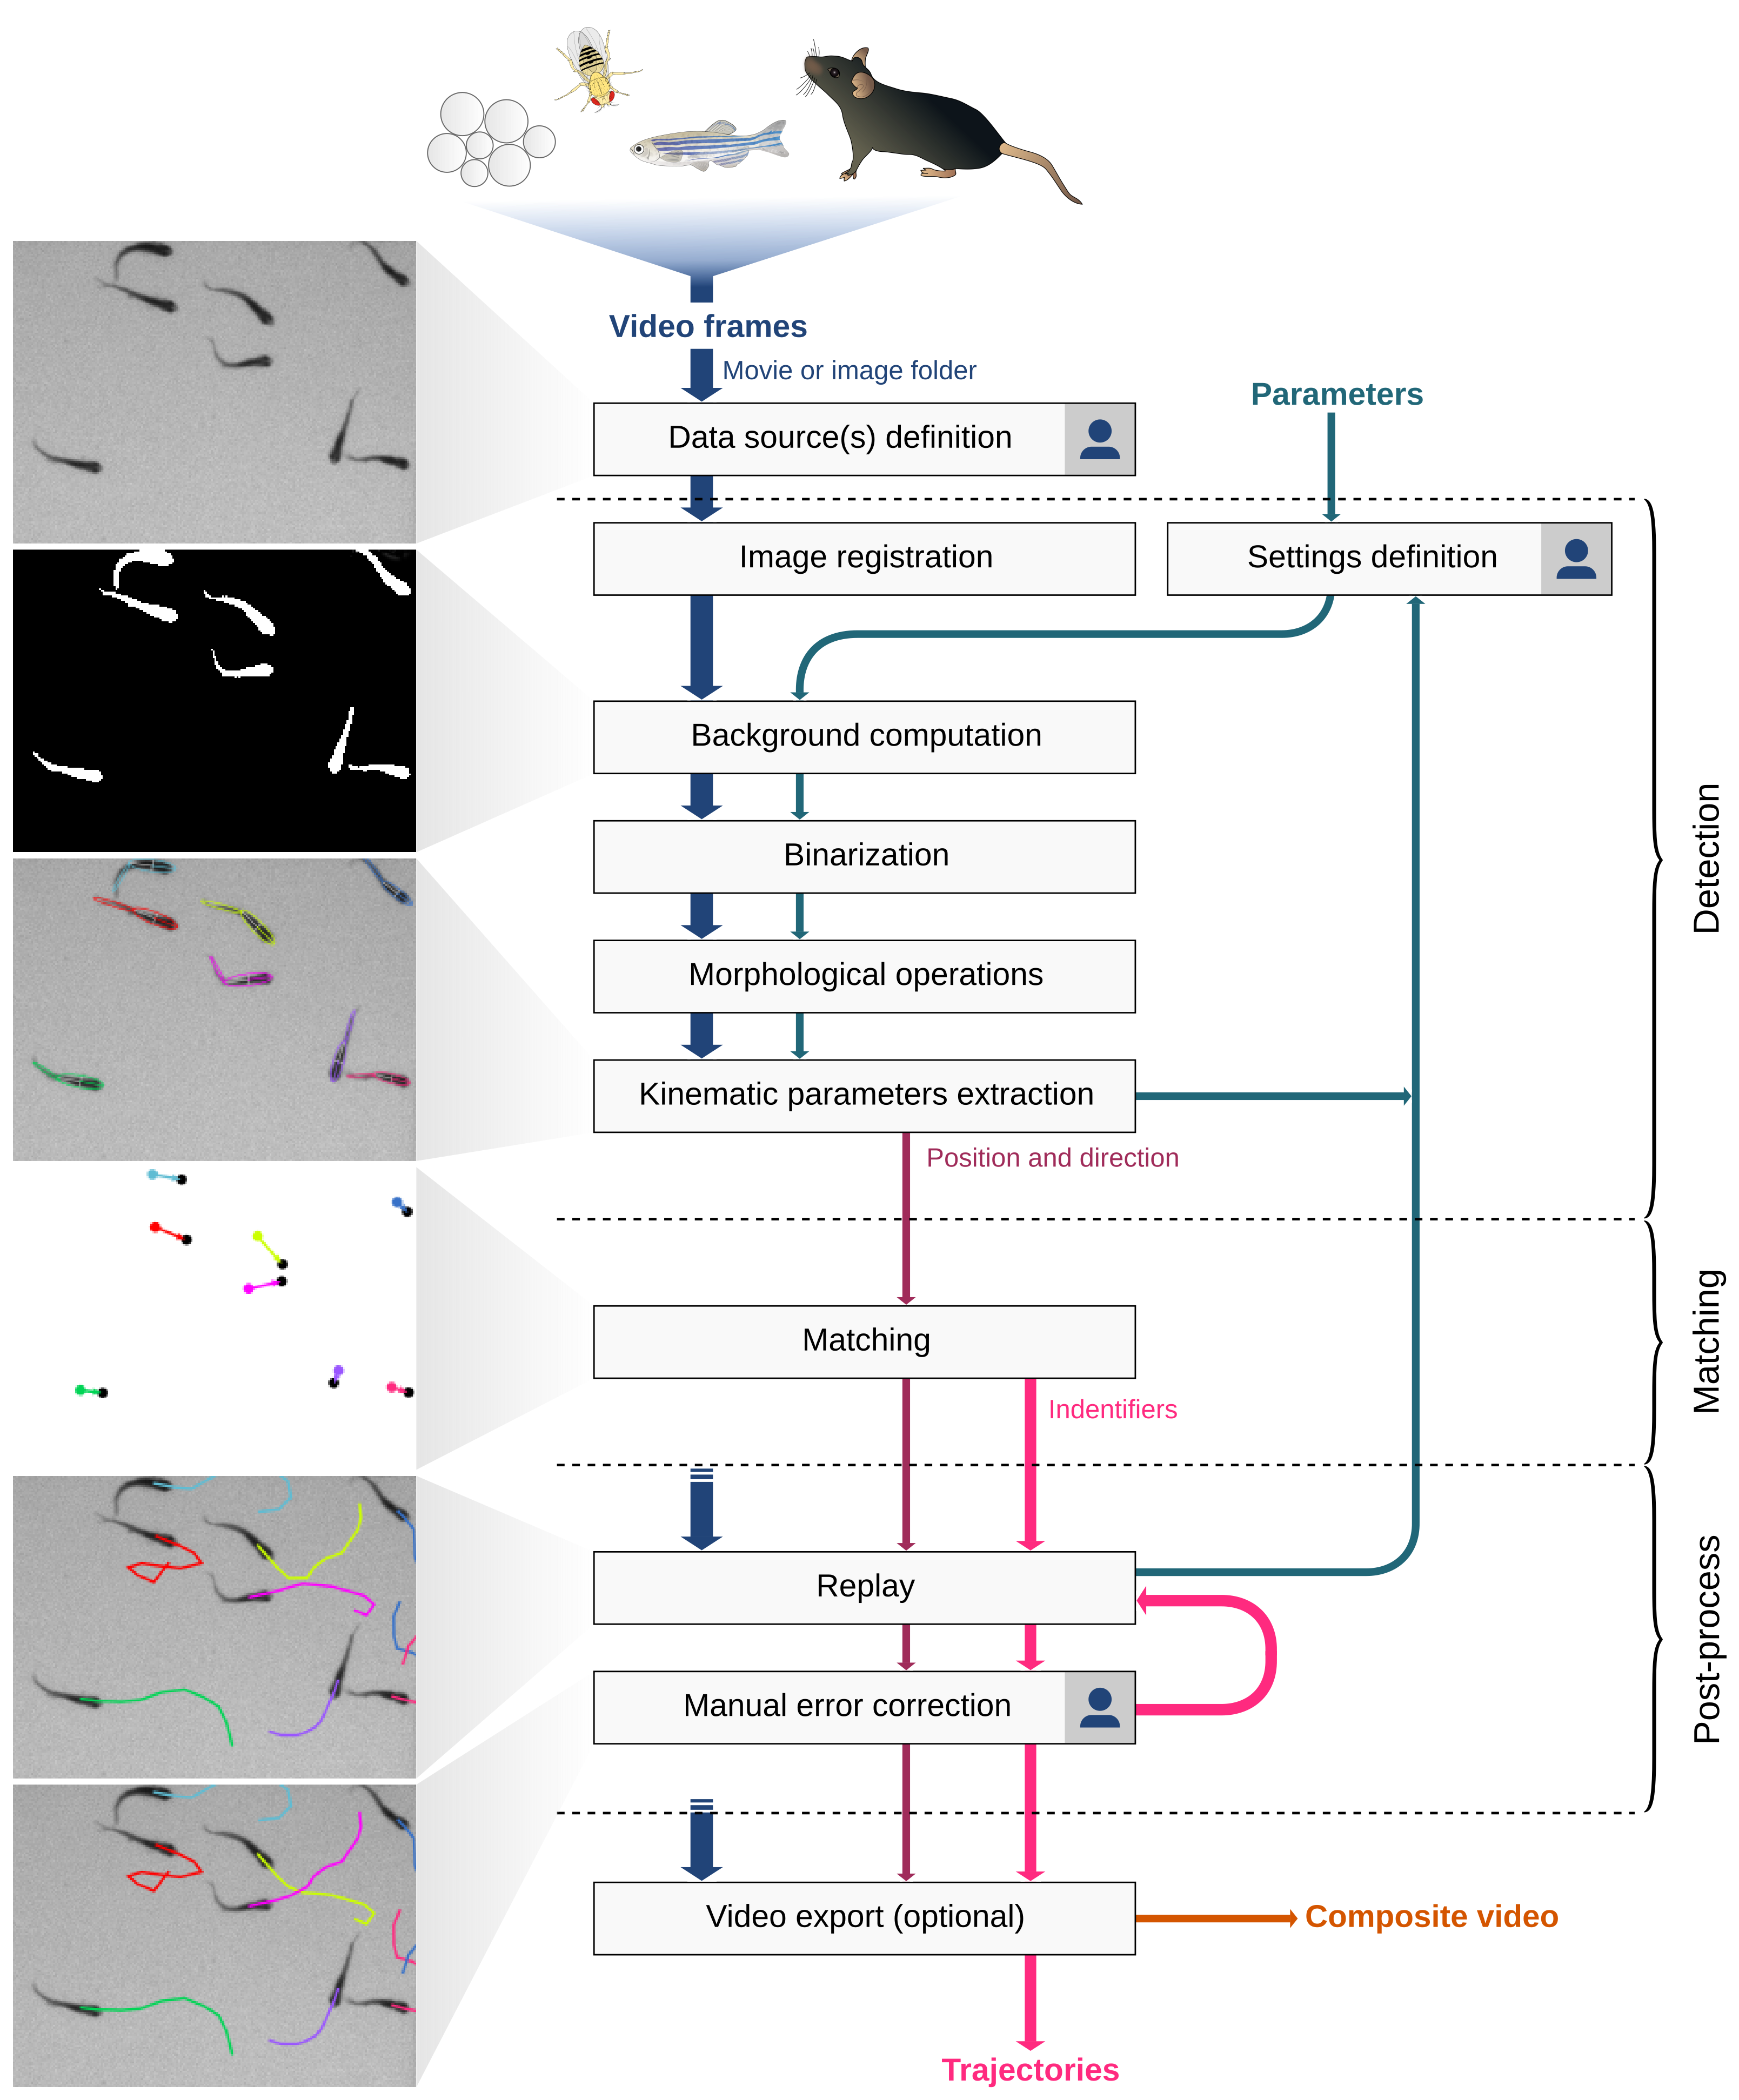
\includegraphics[width=0.75\textwidth]{part_1/assets/Figure_1.png}    
    \caption{\textbf{FastTrack flux de traitement.} Il se divise en trois parties distinctes : la détection, l'association et le post-traitement.}
    \label{part_1:fig_1}
    \end{figure}
	
	
		\subsection{Détection}
		
		L'étape de détection a pour but d'extraire les paramètres cinématiques de chaque objet qui seront ensuite utilisé dans l'étape d'association. FastTrack inclut une collection de filtres d'analyse d'images permettant à l'utilisateur d'optimiser la détection des objets sans avoir à recourir à un logiciel externe.
		
		
		\paragraph{Calcul du fond}
		Chaque analyse commence par calculer une image de fond. Si l'utilisateur possède déjà une image de fond préalablement enregistré, il peut directement l'ouvrir dans le logiciel. Sinon trois méthodes de calcul sont possibles :
		\begin{itemize}
			\item Projection du maximum d'intensité.
			\item Projection du minimum d'intensité.
			\item Projection de la moyenne d'intensité.		
		\end{itemize}
		Les trois méthodes reposent sur le même principe. L'utilisateur choisit $n$ images dans la séquence, le logiciel va projeter dans la direction perpendiculaire à l'image soit le maximum, soit le minimum ou bien la moyenne de la séquence. En pratique, on projettera le maximum (resp. minimum) si les objets sont plus foncés (resp. clairs) que le fond de manière à faire disparaître les objects et ainsi obtenir le fond. L'utilisateur peut effectuer une registration de chaque images avant projection de manière à corriger un éventuel mouvement de la caméra.
		
		
		\paragraph{Registration}
		L'utilisateur peut choisir d'effectuer une registration des images, trois méthodes sont proposées dans le logiciel. Chaque méthode est implémenté de manière pyramidale, c'est à dire que la registration est d'abord effectuée sur une image dégradée pour corriger de manière grossière le déplacement, puis la correction est affinée en augmentant la qualité de l'image jusqu'à arriver à l'image originel. Cela permet d'accélérer le processus, la registration étant souvent un procédé relativement coûteux en temps de calculs.\\
		
		La première méthode proposé est la corrélation de phase. Elle permet de corriger les mouvements de translation entre deux images en utilisant le théorème de Fourier dans le domaine fréquentiel. Cette méthode est très rapide mais reste limité à de petits mouvements de translation uniquement.\\
		
		La deuxième méthode proposées est la méthode Enhanced Correlation Coefficient (ECC). Dans FastTrack, elle est restreinte à corriger les mouvements de translation et de rotation uniquement. Elle consiste à utiliser le coefficient de corrélation comme mesure pour trouver la meilleure transformation entre deux images. Cette méthode a pour avantage d'être relativement rapide, le problème d'optimisation non linéaire pouvant être résolue de manière linéaire. Elle est performante pour des images bruités et ayant des distorsions photométrique (contraste, luminosité).\\
		
		La troisième méthode est une méthode basée sur le repérage de points clefs. Elle permet de corriger les mouvements et les déformations (homographie). Les points clefs (environ 500) sont automatiquement déterminé sur deux images grâce à l'algorithme ORB. Ces points sont ensuite associés deux à deux en utilisant l’algorithme RANSAC permettant de trouver la meilleure transformation entre les deux images. Cette méthode, plus précise nécessite une qualité d'image suffisante pour pouvoir discerner des points clefs.
		
	\begin{figure}[h]
    \centering
    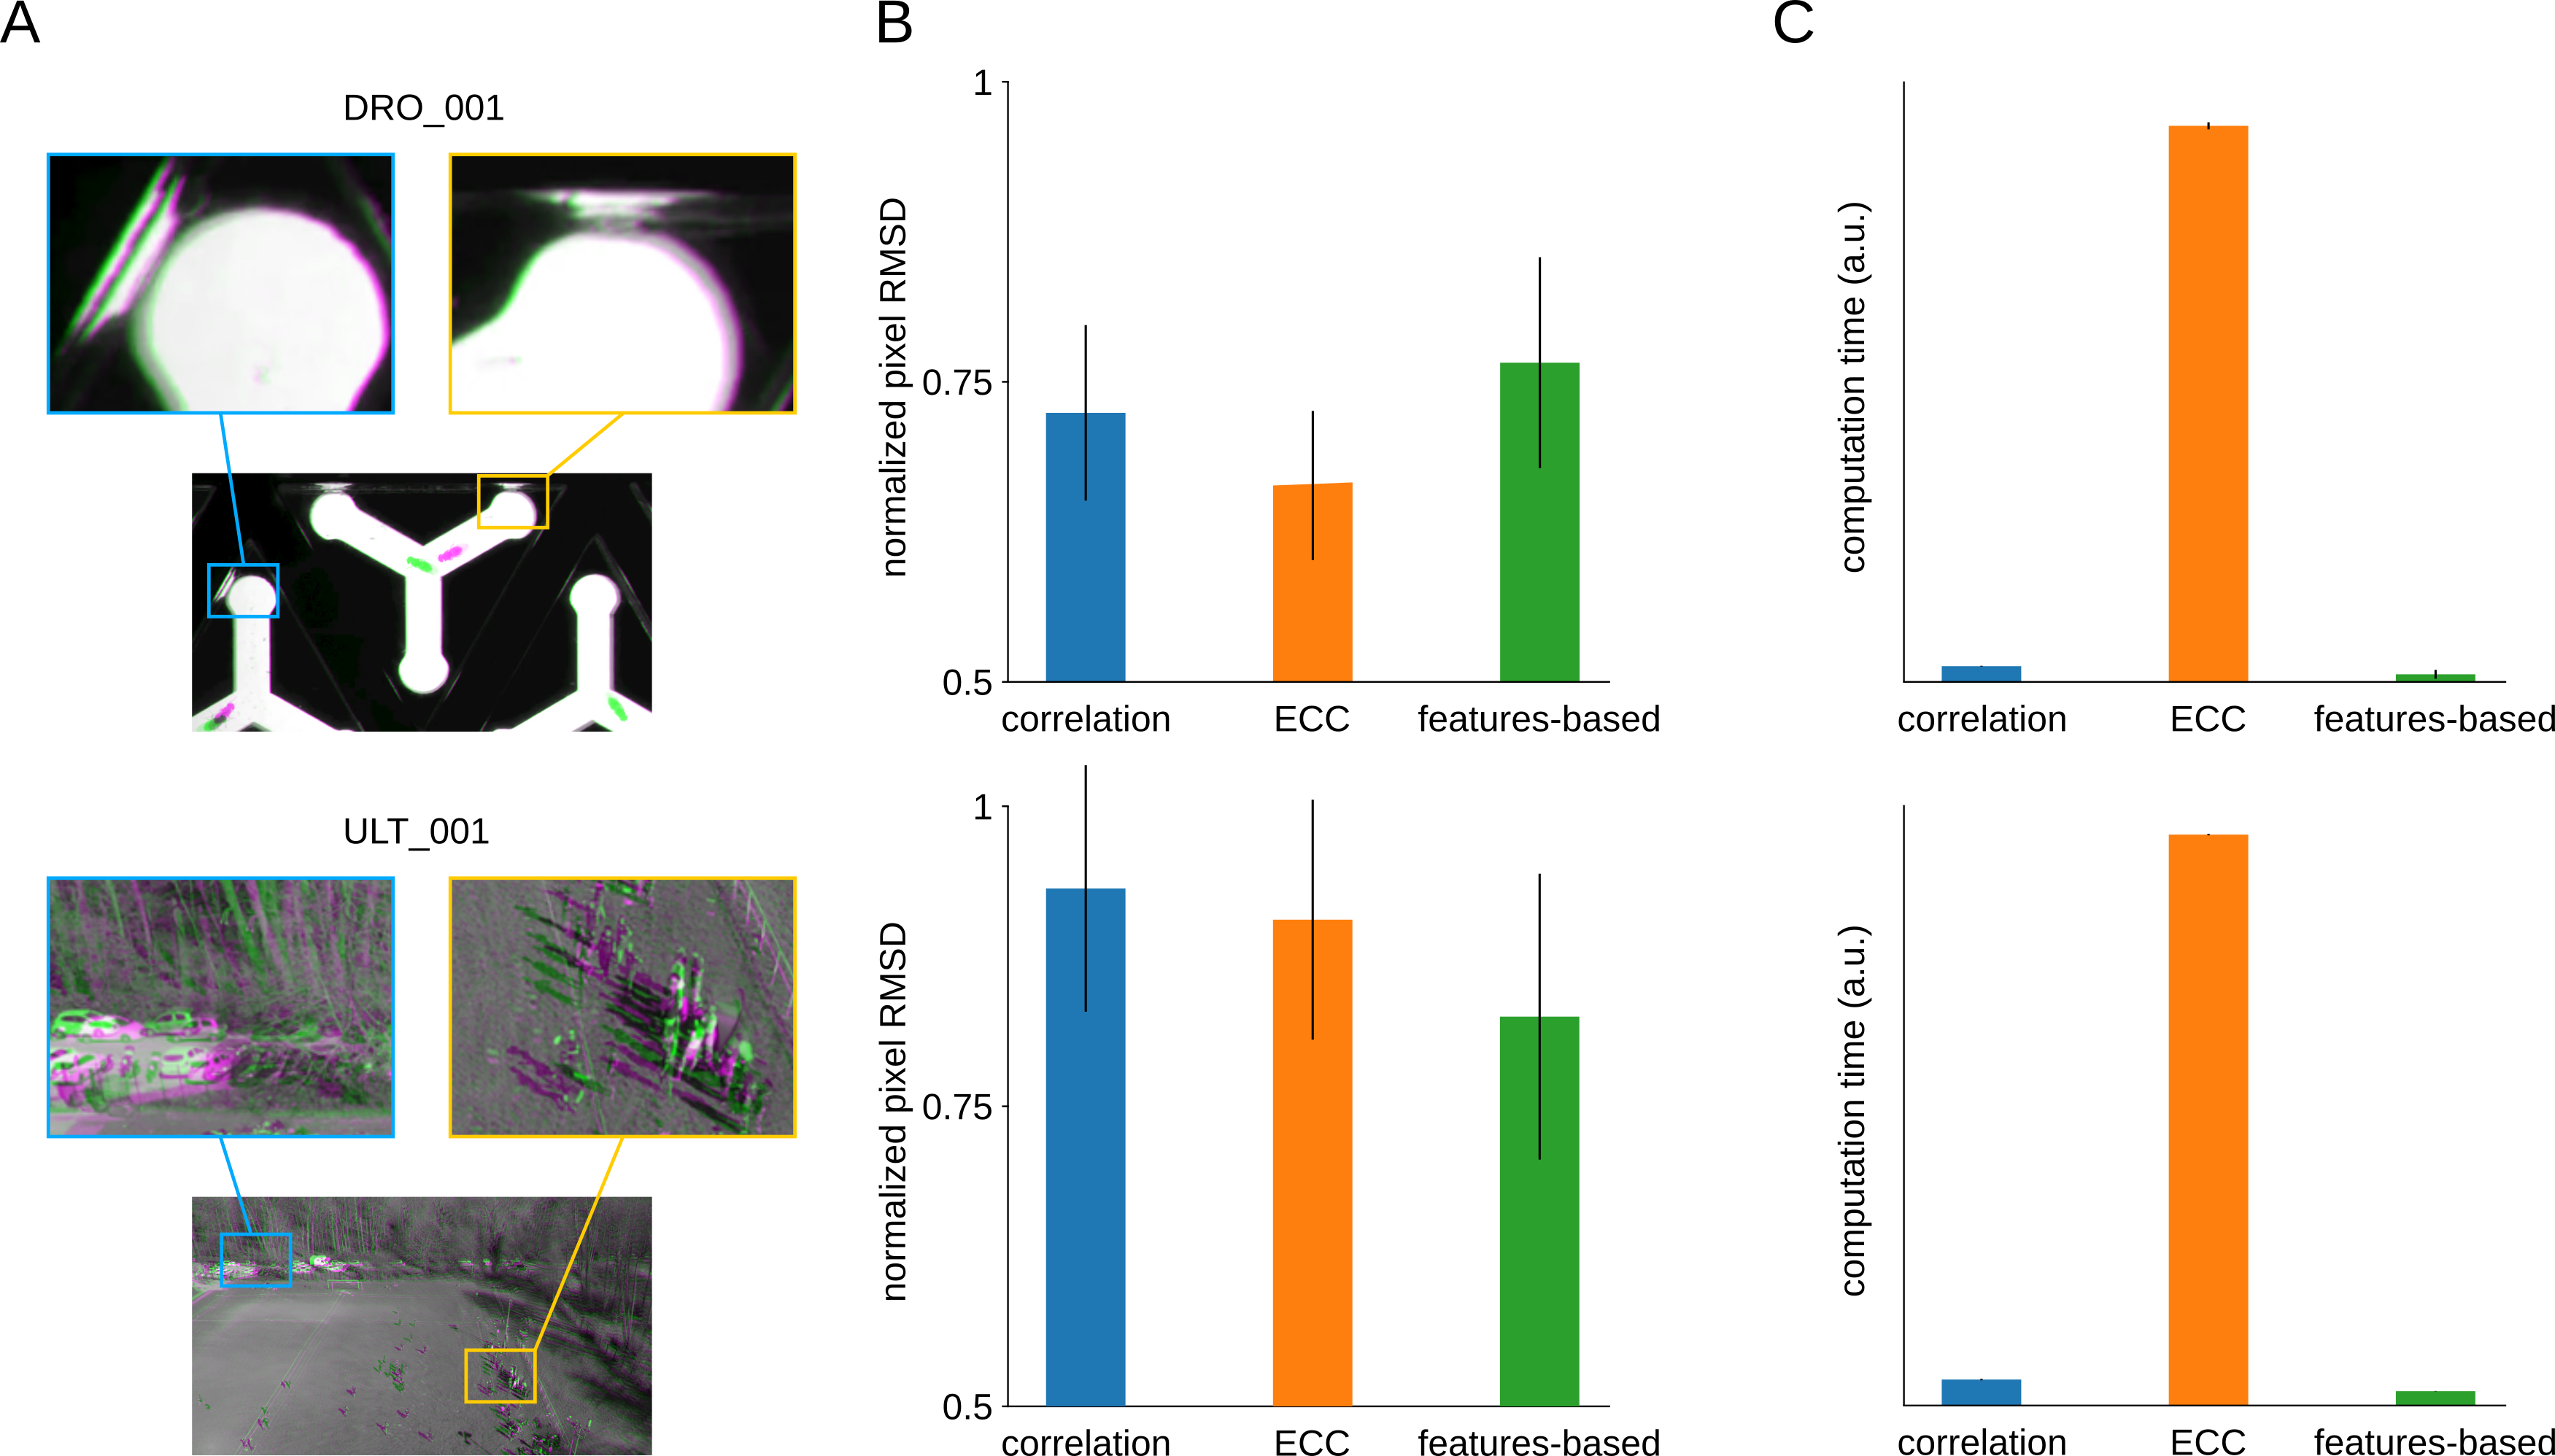
\includegraphics[width=1\textwidth]{part_1/assets/Figure_2.png}    
    \caption{\textbf{Registrations.} Deux films avec une dérive sévère sont utilisés comme référence (DRO\_001 en hautn ULT\_001 en bas). (\textbf{A}) Comparaison entre une image (magenta) avec la première image (vert), avec agrandissement des détails en insert. (\textbf{B}) Déviation moyenne carrée (RMSD) de l'intensité des pixels avant et après registration, moyennée sur toutes les images et normalisée par la RMSD sans registration pour les trois méthodes. Barres d'erreur : déviation standard. (\textbf{C}) Temps moyen relatif pour les trois méthodes (unités arbitraires). Barres d'erreur : déviation standard.}
    \label{part_1:fig_2}
    \end{figure}
		
		
		\paragraph{Binarisation}
		Chaque image est ensuite binariséecd  en y soustrayant l'image de fond puis en définissant une valeur seuil. Dans le mode interactif, l'utilisateur peut voir l'impact des paramètres sur l'image binarisée ce qui permet d'ajuster facilement le seuil de binarisation. Le logiciel détecte également si le fond est plus foncé (resp. clair) que les objets permettant d'avoir à la fin de cette opération une image binaire  où les pixels appartenant à l’objet sont égaux à  et les pixels appartenant au fond sont égaux à 0.
		
		
		\paragraph{Opération morphologique}
		Un ensemble d'opérations morphologiques (dilatation, érosion, ouverture etc...) peut-être effectué sur l'image binaire pour améliorer la détection et éliminer d'éventuels artefacts. Différentes formes et tailles de kernels sont disponibles.
		
		
		\paragraph{ROI}
		L'utilisateur peut sélectionner une région D’intérêt et exclure le reste de l'image de l'analyse. Cela permet d'accélérer le processus d'analyse et d'éviter la détection d’objets parasites. En mode interactif, cette ROI peut être dessiné directement sur l'image.
		
		
		\paragraph{Tri}
		Pour exclure les objets trop petits correspondant à du bruit ou trop gros comme par exemple deux objets superposés, l’utilisateur doit sélectionner deux tailles caractéristiques. En mode interactif, les objets sont coloriés soit en rouge, soit en vert suivant si leur taille appartient à la gamme de tailles sélectionnée.
		
		\paragraph{Extraction des paramètres cinématique}
		Sur la base des images binaires, le logiciel va détecter le contour de chaque objet. Une étape importante de toutes procédure de tracking est l'extraction des paramètres qui serviront dans l'étape d'association. C'est en générale dans le choix de ses quantités que les algorithme de tracking diffère pour se spécialiser à un type d'objet donné. Dans FastTrack, les paramètres extraient sont la positions du centre de masse ainsi que l'orientation de l’objet, dans quantité rapidement calculées et assez généralistes pour s'adapter à une grande diversité de type d'objets.\\
		
		Pour cela, FastTrack calcule l'ellipse équivalente de l'objet à partir des moments d'ordre deux de l'image binaire. Cette procédure est accélérée en utilisant directement le contour grâce à la formule de Green. L'orientation de l'objet est donnée par l'axe majeur de l'ellipse équivalente. Sa direction est déterminée en projetant chaque pixel de l'objet sur l'axe majeure de l'ellipse. On calcule ensuite la skewness de la distribution des distances des points projetés par rapport au centre de masse. Le signe de la skewness est un indicateur robuste de l’asymétrie de l'objet par rapport à son axe majeure à partir de laquelle on peut déterminer la direction de l'objet.\\
		
		Pour les objets déformables, la direction calculer précédemment peut être différente de la direction de déplacement de l'objet. Par exemple dans le cas du poisson zèbre, celui-ci déforme son corps de manière périodique pour se déplacer, seul la tête est dirigée dans la même direction que le mouvement. C'est pourquoi on décompose l'objet en deux ellipses équivalentes, l'utilisateur peut alors choisir quelle ellipse représente le mieux la direction de déplacement.
		
		
		\subsection{Association}
		
		L'étape d'association a pour but de conserver l'identité des objets d'une image sur l'autre. Pour se faire, FastTrack utilise une méthode dérivée de ?, qui tire partie du fait que la position et la direction de chaque objet change très peu d'une image sur l'autre.
		Pour chaque pair d'objet (i,j) appartenant à deux images successives, deux coûts sont calculés.
		Le coût "dur" calculé comme suit :
        $$
        \left\{
        	\begin{array}{ll}
        		h_{i,j} = 1 & \mbox{si } r_{i,j} < h_{d} \\
        		h_{i,j} = \inf & \mbox{sinon }
        	\end{array}
        \right.       
        $$
        avec $r_{i,d}$ la distance entre les objets i et j, $h_{d}$ un seuil qui représente la distance maximale de déplacement autorisée entre deux images successives.
		Le coût "mou" calculé comme suit:
		$$
        c_{i,j} = \frac{r_{i,j}}{s_d} + \frac{\delta\alpha_{i,j}}{s_{\alpha}}		
		$$
		où $\delta\alpha_{i,j}$ est la valeur absolue de la différence angulaire entre les directions de i et j, $s_{d}$ et $s_{\alpha}$ sont des coefficients de normalisation qui représente un déplacement et une réorientation typique du système étudié entre deux images successives.
		Ces deux coûts sont ensuite multipliés élément par élément pour donner la matrice suivant :
		$$
        C_{i,j} = \left\{
        	\begin{array}{ll}
        		c_{i,j} & \mbox{si } r_{i,j} < h_{d} \\
        		\inf & \mbox{sinon }
        	\end{array}
        \right.       
        $$
		La matrice de coup peut être rectangulaire si le nombre d'objets n'est pas constant comme lors d'occlusion ou d'ajout d'objets. Un paramètre de mémoire peut être sélectionner de manière à ne plus pouvoir assigner les objets si ceux-ci on disparu depuis plus de $n$ images.
		Le meilleure association est celle dont la somme des coûts est minimale. Ce problème est appelé "the rectangular assignement problem" et peut être résolu de manière exacte en utilisant l’algorithme hongrois, FastTrack utilise l'implémentation Kuhn-Munkres en C++ pour résoudre rapidement ce problème.
		
		\subsection{Post-traitement}
		
		\paragraph{Correction manuelle}
		FastTrack intègre un outil de correction manuel du tracking. Une fois une analyse terminée, le résultat peut être affiché dans une interface ergonomique créée à cet effet. L'utilisateur peut rejouer le film en y surperposant les résultats de l'analyse, il peut sélectionner un objet pour en consulter les paramètres (aire, contour, identité, etc...). L'utilisateur peut aussi directement corriger les erreurs en supprimant des objets ou en échangeant l'identité des objets. Cette interface est concu dans un soucis d'ergonomie et de performance. Des raccourcis claviers ainsi qu'une sélection à la volé des objets directement en cliquant sur la vidéo permette à l'utilisateur de rapidement vérifier et corriger les analyses. Il est aussi possible d'enregistrer, en plus des données brutes d'analyse, un film avec les résultats du tracking superposés.
		Cette interface de correction manuel permet de déplacer la charge de travail qui est traditionnellement placé sur le pré-traitement des données, vers le post-traitement. Le logiciel reste alors général et peut s'adapter à une grande diversité d'objets et performant grâce à une interface spécialement pensée pour réduire le temps de post-traitement.
		
		\paragraph{Analyse}
		L'analyse statistique des données n'est pas implémenté dans FastTrack. Après chaque analyse, le logiciel génère un dossier contenant les résultats. Le fichier principal est nommé tracking.txt et il contient les données brutes de l'analyse avec une image et un objet par ligne. Ce format est compatible avec tous les logiciels d'analyse les plus utilisés (R, Python, MATLAB), des exemples sont disponibles dans la documentation.
		
	\section{Déploiement}
		\subsection{CI/CD}
		Le déploiement est une partie à ne pas négliger dans la conception d'un logiciel et deux aspects sont tout particulièrement importants à considérer. Du point de vue de l'utilisateur, le logiciel doit pouvoir être installé facilement sur les plateformes supportées. Du point de vue du mainteneur, la partie de déploiement doit être facilement réalisable et reproductible de manière à pouvoir intégrer rapidement les correctifs et nouvelles fonctionnalités développées. C'est dans cette optique que FastTrack suit la philosophie CI/CD en tirant partie du nouveau système GitHub Action.\\
		
		L'intégration continue (CI) est un ensemble de pratiques qui a pour but d'intégrer rapidement les changements au projet de manière automatisée. Elle est couplée avec une automatisation des tests unitaires. FastTrack tire partie du système CI/CD de GitHub nommé Action, à chaque nouveau changement (commit\footnote{Action d'envoyer la liste de modifications effectuées dans le système de gestion de version}) ou nouvelle collaboration (pull-request \footnote{Action de demander l'ajout de modifications effectuer dans une branche au projet}), une série de tests est automatiquement déclenchée. Ces tests vont vérifier le bon fonctionnement de l'algorithme de tracking ainsi que le formatage du code source. Seul les changements qui passent les tests peuvent être intégrés au projet se qui garantie la reproductibilité des analyses ainsi que la cohérence du code source et de la documentation.\\
		
		La livraison continue (CD) quant à elle automatise la livraison du logiciel dans sa forme finale. Elle permet d'intégrer rapidement les changements au logiciel sans avoir à le faire manuellement pour chaque plateforme supportée. Dans le cas de FastTrack, le CD est implémenter grâce à GitHub Action et une nouvelle version du logiciel est compilée pour Linux, MacOs et Windows à chaque nouveau commit qui est intégré à la branche principale. Des version stables du logiciel sont quand à elle compilée à chaque palier de développement. Ce système est un gain de temps majeur pour un logiciel multi-plateformes comme FastTrack, et il permet à l'utilisateur de toujours disposer des derniers correctifs et des dernières fonctionnalités.\\
		
		FastTrack supporte nativement les trois plateformes majoritairement utilisées : les systèmes Linux avec une AppImage qui supportent toutes les distributions et un PPA pour Ubuntu uniquement, Windows avec un installateur, MacOS avec une App. La dernière version stable peut-être téléchargé sur le site web http://www.fasttrack.sh, la dernière version CD sur https://github.com/bgallois/FastTrack/releases. La procédure pour compiler soit même le logiciel est disponible dans la documentation du développeur pour les autres plateformes.
		
		\subsection{Documentation}
		Une documentation extensive est disponible, elle se sépare en deux parties : une à l'usage des utilisateurs et une autre à l'usage des développeurs.
		
		\paragraph{Utilisateur} La documentation utilisateur est disponible à l'adresse https://www.fasttrack.sh/UserManual/docs/intro.html. Cette documentation est mise en forme à partir du logiciel Docusaurus et les utilisateurs peuvent y contribuer https://github.com/bgallois/FastTrack/. Elle regroupe l'ensemble des informations nécessaires à l'utilisation du logiciel ainsi que des vidéos d'explication pour aider à prendre le logiciel en mains.
		
		\paragraph{Développer} La documentation du développeur est disponible à l'adresse https://www.fasttrack.sh/API/index.html. Elle est automatiquement générée grâce au logiciel Doxygen à partir de la documentation présente dans le code source de FastTrack. Elle regroupe l'ensemble des informations nécessaires aux développeurs voulant modifier ou contribuer à FastTrack.

		
\chapter{Base de données de films}
    
    Pour démontrer que FastTrack peut être utilisé pour analyser des films provenant d'une grande diversité de systèmes, nous avons compilé une base de données de films nommée $TD^2$. Cette banque de films peut être téléchargé à l'adresse suivante URL. Les films proviennent soit de données déjà publiées dans la littérature, soit ils nous ont été fourni par les auteurs eux-mêmes sous licence CC-BY-NC-SA. Chaque film est identifié par un code à 3 lettres définissant le système (ex. ACT : active matter, ZFA : zebrafish adult etc...) et 3 chiffres pour indexer les films provenant de systèmes identiques. $TD^2$ regroupe actuellement 41 films comprenant différent types d'objets de nature et de taille très différents : 7 espèces d'animaux allant du poisson à la mouche, des cellules, des particules actives, des gouttes microfluidiques ainsi que des objets macroscopiques tels des joueurs d'ultimate ou des voitures. Une vidéo donnant un rapide aperçut de tous les systèmes utilisés est disponible à l'adresse suivante URL.\\

    Un autre aspect important à considérer est le nombre d'objets par film ainsi que leurs éventuelles apparitions, disparitions et chevauchements. Dans 22 films sur 41, le nombre d'objets est variable et des objets sortent ou rentrent dans le champ de la caméra durant l'enregistrement. Dans 19 films sur 41, des objets peuvent se chevaucher créant un phénomène d'occlusion que le logiciel doit gérer pour retrouver l'identité des objets.

	\begin{figure}[h]
    \centering
    \includegraphics[width=1\textwidth]{part_1/assets/Figure_td2.png}    
    \caption{\textbf{$TD^2$.}}
    \label{part_1:fig_5}
    \end{figure}


\chapter{Résultats}

	\section{Analyse de la base de données}

  Analyser des films provenant de systèmes aussi diffèrent que ceux compilés dans $TD^2$ est un véritable challenge. Cela est dû en partie aux conditions d'enregistrement qui peuvent être très diverses et qui complexifient la tâche de détection des objets. Deux difficultés récurrentes sont à soulever : les variations de l'illumination (ex. réflexion dans GRA\_001, ombres dans SOC\_001) et le chevauchement des objets (ex. HXB\_001).
  Dans le cas de films provenant du milieu académique, les systèmes sont souvent conçus pour limiter ou contourner ces deux difficultés. Il est commun de trouver des films dont l'illumination est uniforme et constante. de même un confinement quasi-2D ainsi qu'un nombre d'objet restreint dans le champ de la caméra permettent de réduire le nombre d'occlusions.
  Dans $TD^2$, 23 films ont une illumination assez bonnes pour être analysés directement avec FastTrack, les autres ayant dû subir un pre-processing individuel spécifique avant de pouvoir être analysées. Deux films ayant un nombre d'occlusions extrêmement élevé ont été écarté (HXB\_001 and ZFL\_001) car ne pouvant pas être analysé avec le logiciel.
  Les 39 films restant ont pu être analysés avec FastTrack sans difficulté. L'algorithme de Kuhn-Munkres étant de complexité $O(n^3)$ le temps de calcul est en général assez rapide. Sur l'ordinateur utilisé pour l'analyse (ordinateur de bureau moderne), on observe une vitesse d'analyse pouvant aller jusqu’à 500 images/secondes. Les films les plus volumineux en taille et nombre d'images et en nombre d'objets n'ont pas pris plus de quelques dizaines de minutes. Chaque film a ensuite été corrigé manuellement grâce à l'outil intégré dans le logiciel.
	
	\section{Estimation de la charge de travail de correction}
	
	FastTrack est conçu pour que la phase de post-traitement soit la plus faible possible, mais cette charge de travail varie grandement suivant les films analysés. On va ici montrer que cette charge de travail peut être estimée rapidement pour un film donnée. On assumera pour la suite que la détection et l'association ont déjà été réalisées.\\
	
	La méthode repose sur l'évaluation de la probabilité d'incursion $P_{inc}$. Une incursion étant définie par la sortie d'un objet de sa cellule de Voronoï, prise en $t_1$, durant un trajet entre $t_1$ et $t_2$. Le nombre d'incursions dépend de la distribution des déplacements, de la densité d'objets, de la géométrie de la cellule de Voronoï et du degré d'alignement des déplacements. On peut écrite cette probabilité :
	$$$$
	où $\rho=r\sqrt{d}$ est le déplacement réduit adimensionné, $R(\rho)$ la distribution des $\rho$ et $p_{inc}(\rho)$ la probabilité géométrique d’incursion qui ne dépend que des propriétés géométrique de la disposition des objets. On calcule $p_{inc}$ en prenant les cellules de Voronoï de tous les objets sur toutes les images, puis en déterminant la proportion des angles pour lesquels un déplacement de $\rho$ implique un incursion dans une cellules de Voronoï voisine. Intuitivement, on peut se convaincre que $p_{inc}$ va de 0 quand $\rho->\inf$, à 1 quand $\rho>>1$. La forme de cette fonction est sensible à la densité des objets, compacts (ex. ACT\_002), clairsemés (ex. PAR\_001), et à la taille globale du système quand celui-ci est restreint par des murs (ex. ZFA\_001).\\
	
	Les distributions de $\rho$ et $p_{inc}$ sont représentées figure~\ref{} pour trois films de $TD^2$ représentatifs de trois systèmes très différents. Il n'est pas nécessaire d'avoir un tracking parfait pour avoir une bonne estimation de cette valeur car les quelques erreurs possibles ont une influence marginale sur la distributions des $\rho$ donc sur $P_{inc}$.\\
	On a calculé $P_{inc}$ pour tous les films de $TD^2$ figure~\ref{}, de manière à en estimer le nombre d'incursion $n_{inc}$ :
	$$
	    n_{inc}=P_{inc}*N_{obj}
	$$
	avec $N_{obj}$ le nombre total d'objet dans le films.
	Chaque incursion ne résultant pas à une inversion de l'identité de deux objets, donc à une erreur, on gardera en tête que cette valeur représente la borne maximale possible d'erreurs. Dans $TD^2$, seulement 5 films on $n_{inc}>1$ ce qui suggère que pour la grande majorité des films, le post-traitement se résume à un simple contrôle. Les 5 films restants sont connus pour leur difficulté à analyser dont 2 (ACT\_003 et ACT\_004) ont nécessités le développement d'un algorithme spécifique, 2 autres (BAC\_001 et ZFA\_001) des logiciels dédiés pour être analysés.
	
	\begin{figure}[h]
    \centering
    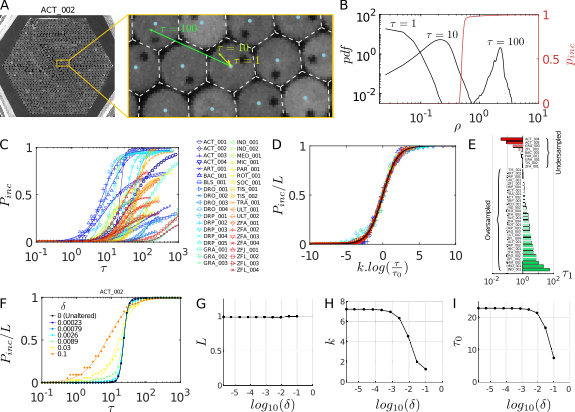
\includegraphics[width=1\textwidth]{part_1/assets/Figure_3.png}    
    \caption{\textbf{Probabilité d'incursion} (\textbf{A}) Définition des incursions : objets faisant de petits déplacements à l'intérieur de leurs cellules de Voronoï (haut), grands déplacements générant des incursions dans les cellules de Voronoï voisines (bas). De telle incursions sont susceptibles de générer des erreurs de tracking. (\textbf{B}) Images extraient de 3 films avec le déplacement instantané des objets (rouge). La position initiale est marqué d'un point. (\textbf{C}) Probabilité géométrique d'incursion $p_{inc}$ en fonction du déplacement normalisé $\rho$ (noir) et de la densité de probabilité de $\rho$ (rouge) pour les trois films correspondant. La probabilité d'incursion $P_{inc}$ correspond à l'aire de recouvrement des deux courbes. (\textbf{D}) Probabilité d'incursion $P_{inc}$ (bleue) et nombre d'incursion $n_{inc}$ (orange) pour 19 films de $TD^2$. Le reste des films ayant $P_{inc}<10^{-20}$}
    \label{part_1:fig_3}
    \end{figure}
	
	\section{Optimisation des paramètres}
	
	L'optimisation des paramètres d'analyse peut parfois s'avérer être une tâche délicate, on présentera ici une méthode basée sur la minimisation du nombre d'inversion d'identités (swap). Les étapes suivies pour le calcul sont présentés figure~\ref{}. Pour compter le nombre d'inversions, il est seulement nécessaire d'avoir un seul film du système étudié parfaitement analysé, ce qui peut être réalisé par un post-traitement méticuleux. On peut ensuite définir la probabilité d'inversion $P_{swap}$ et varié la paramètre afin de la minimiser. Pour se faire, on utilisera l'interface en ligne de commande FastTrack\_cli qui permet d'appeller FastTrack directement à l'intérieur d'un script Python pour automatiser la minimisation. On définit la probabilité d'inversion :
	$$
	    P_{swap}=\frac{N_{swap}}{N_{obj}-n_{ap}}
	$$
	avec $N_{swap}$ le nombre total d'inversions, $N_{obj}$ le nombre total d'objets sur toutes les images, et $n_{ap}$ le nombre de fois qu'un nouvel objet apparaît. Si le nombre d'objets est constant et noté $n$, alors $n_{ap}=n$ et $*N_{obj}=nT$ avec $T$ le nombre d'images dans le film, alors on peut simplifier $P_{swap}$ :
    $$
	    P_{swap}=\frac{N_{swap}}{n(T-1)}
	$$
	On a étudier en premier lieu l'impact du paramètre $h_d$, la distance maximale de déplacement autorisé entre deux images successives. La figure~\ref{} représente l'évolution de $P_{swap}$ en fonction de $h_d$ pour trois films tirés de $TD^2$. On voit que pour un faible $h_d$, $P_{swap}$ est essentiellement donnée par la distribution des déplacements des objets, ce qui s'explique par le fait qu'un grand nombre d'erreurs est générées quand un objet n'est pas autorisé à se déplacer plus qu'on son déplacement typique. Pour des $h_d$ grands, c'est la distribution des distances aux voisins (défini par la tesselation de Voronoï) qui influence le plus $P_{swap}$, algorithme devenant plus sensible aux incursions et pouvant faire plus d'erreurs avec les entrées et sorties du champ de vision.
	Entre ces deux cas extrêmes, il existe en général un minimum, ce qui est particulièrement évident pour les systèmes denses dont la distribution des distances aux voisins est très piquées. Par exemple pour DRP\_001 on voit que $P_{swap}$ tombe à 0 pour un intervalle de $h_d$. La fréquence d'acquisition joue un rôle important ici, pour des films très résolue temporellement, on aura une distribution de déplacement décalée à gauche vers des distances plus courtes, cela va donner une séparation claire et de petite valeurs en $P_{swap}$. Pour des films avec une résolution temporelle médiocre (ZFJ\_001), les deux distributions se recouvrent et $P_{swap}$ reste toujours bloquée à de grandes valeurs.\\
	
	On peut faire une analyse similaire pour les autres paramètres. On a représenté $h_d$ en fonction de $h_t$ (nombre d'image où l'objet disparaît autorisé), on voit qu'on peut trouver une bande de paramètres où $P_{swap}$ est minimale.
	
	Pour résumer, on peut faire cette analyse pour un film parfaitement analysée grâce à FastTrack et à l'outil de post-traitement, puis en dérivé un jeu de paramètre optimaux à appliquer sur des films similaire de manière à réduire la charge de travail en post-traitement.\\
	
	\begin{figure}[h]
    \centering
    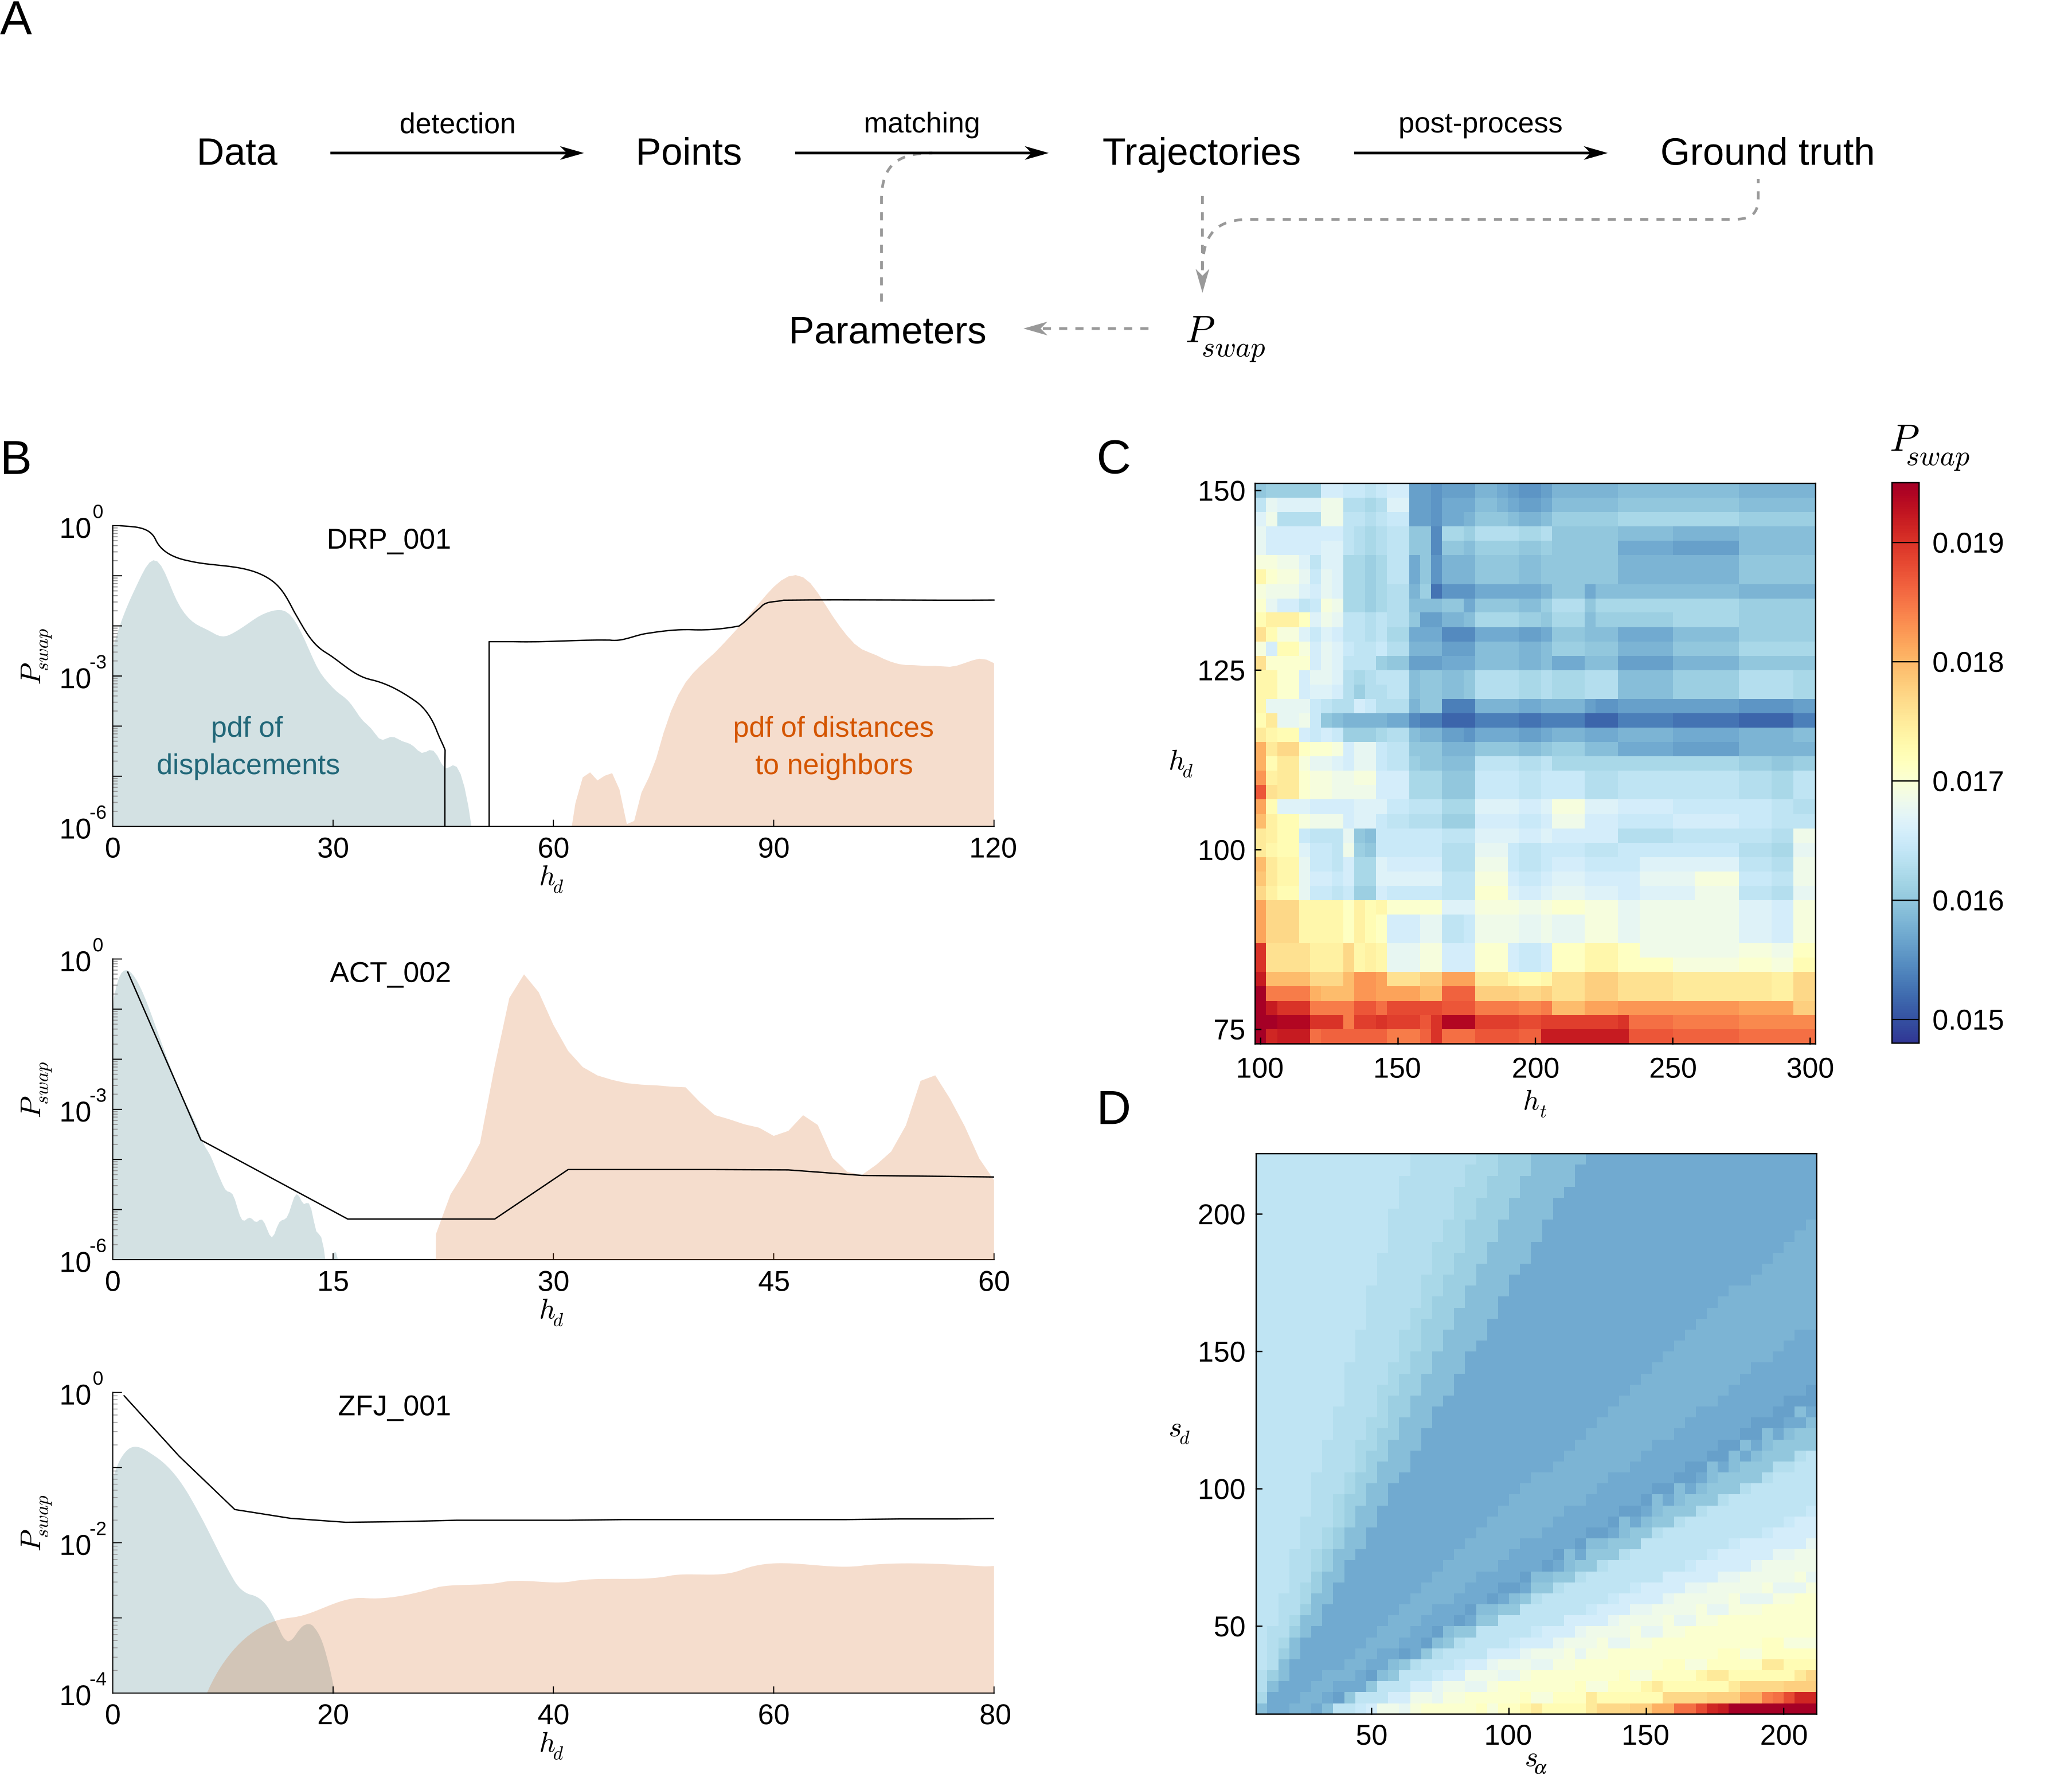
\includegraphics[width=1\textwidth]{part_1/assets/Figure_4.png}    
    \caption{\textbf{Optimisation des paramètres d'analyse basé sur $P_{swap}$} (\textbf{A}) Schéma du workflow d'optimisation : le résultat parfait de tracking est utilisée pour calculer $P_{swap}$ et créer une boucle de rétroaction sur les paramètres d'analyse. (\textbf{B}) $P_{swap}$ (noire) en fonction de la distance maximale $h_d$ (en pixels) pour trois films typiques. Les lignes verticales pour DRP\_001 indique que $P_{swap}$ descend à 0. Les distributions des déplacements entre deux images successives (bleue), et de distance aux voisins (orange) sont montrées pour comparaison. (\textbf{C}) $P_{swap}$ en fonction de la distance maximale $h_d$ et du temps de disparition maximal $h_t$ (en nombre d'images) pour PAR\_001 pour $s_d=95$ et $s_{\alpha}=60$. (\textbf{D}) $P_{swap}$ en fonction de la distance $s_d$ (en pixels) et de l'angle de normalisation $s_{\alpha}$ (en degrés) pour PAR\_001 avec $h_d=210$ et $h_t=90$. } 
    \label{part_1:fig_4}
    \end{figure}
	
	On une autre question souvent posée est de savoir avec quelle résolution temporelle acquérir le film. Une grande résolution permet de diminuer $P_{swap}$ et donc je réduire le post-traitement mais n'est pas toujours envisageable (limitation de la caméra, de l'illumination, nécessité d'un grand espace de stockage).
	Pour étudier l'impact de la fréquence d'enregistrement, on a sélectionné 7 films avec une bonne résolution temporelle et nous les avons dégradés pour à chaque fois calculer $P_{swap}$. tracer en fonction du facteur de dégradation adimentionné $(f-f^{\star})\tau$, on voit que tous les $P_{swap}$ suivent une courbe maîtresse :
	$$
	    L(x)=\frac{1}{1+e^{-1}a}
	$$
	qui est une fonction logistique standard où $f^{\star}$ correspond au facteur de dégradation où $P_{swap}=0.5$, $\tau$ est un facteur de normalisation qui dépend des propriétés dynamique de chaque système.\\
	
	A l'aide de ses résultats, on peut donc proposer un méthode permettant de déterminer la fréquence d'acquisition optimal. Cette méthode nécessite un seul enregistrement de bonne qualité déjà analysé avec FastTrack. Il faut ensuite répété la procédure de dégradation et calculer le $P_{swap}$ résultant. Les $P_{swap}$ peuvent être ajusté à la fonction logitique pour en extraitre les paramètres $f^{\star}$ et $\tau$. Il suffit ensuite de choisir la fréquence d'acquisition en fonction de la quantité de travail que l'utilisateur est prêt à fournir en post-traitement $N_{swap}=P_{swap}(N_{obj}-n_{ap})$.
	
	\begin{figure}[h]
    \centering
    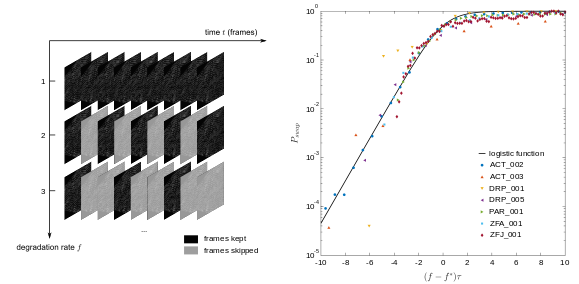
\includegraphics[width=1\textwidth]{part_1/assets/Figure_5.png}    
    \caption{\textbf{$P_{swap}$ et vitesse d’acquisition} (\textbf{A}) Schéma de la procédure de dégradation. (\textbf{B} $P_{swap}$ en fonction du taux réduit de dégradation $(f-f^{\star})\tau$ pour 7 systèmes très différents. $f^{\star}$ et $\tau$ ont été déterminés par un ajustement sur la fonction logistique standard (noire).}
    \label{part_1:fig_5}
    \end{figure}
	
\chapter{Perspective}

	On a vu dans cette partie le logiciel FastTrack. On a détaillé les outils utilisés ainsi que l'implémentation en elle-même. On a ensuite testé le logiciel sur une grande quantité de films présentant des systèmes extrêmement variés et évalué sa performance. On a décrit deux méthodes permettant de trouver facilement les paramètres optimaux d'analyses et la fréquence d'acquisition optimale qui permet de guider l'utilisateur de la conception de l'expérience jusqu'à l'analyse des films.\\
	
	On a aussi abordé un point central du logiciel qui est son appartenance au mouvement open-source. Les codes du logiciel sont entièrement disponible à l'adresse URL. Cela permet d'une part de collaborer au projet pour régler des bugs où ajouter des fonctionnalité. D'intégrer tout ou une partie du projet dans un logiciel ou une expérience déjà existante. Cela renforce la pérennité du projet qui ne dépend pas d'une seule personne pour rester à jour. Enfin la mise en place de la livraison continue (CD) permet de s'affranchir d'une personne dédié à la création de chaque version pour les trois plateformes supportées et donc de réduire le temps nécessaire à la parution de correctifs.\\
	
	La collaboration pour implémenter de nouvelles fonctionnalités, participer à la documentation ou régler des bugs est encourager et peut se faire grâce au système de pull-request de GitHub. Le logiciel à d'abord été testé au sein du laboratoire où il a assez vite été adopté. Il compte à cette date (avant publication de l'article) plus de 500 téléchargements et une base d'une dizaine d'utilisateurs quotidiens.
	
	

